% Options for packages loaded elsewhere
\PassOptionsToPackage{unicode}{hyperref}
\PassOptionsToPackage{hyphens}{url}
\PassOptionsToPackage{dvipsnames,svgnames,x11names}{xcolor}
%
\documentclass[
  letterpaper,
  DIV=11,
  numbers=noendperiod]{scrartcl}

\usepackage{amsmath,amssymb}
\usepackage{iftex}
\ifPDFTeX
  \usepackage[T1]{fontenc}
  \usepackage[utf8]{inputenc}
  \usepackage{textcomp} % provide euro and other symbols
\else % if luatex or xetex
  \usepackage{unicode-math}
  \defaultfontfeatures{Scale=MatchLowercase}
  \defaultfontfeatures[\rmfamily]{Ligatures=TeX,Scale=1}
\fi
\usepackage{lmodern}
\ifPDFTeX\else  
    % xetex/luatex font selection
\fi
% Use upquote if available, for straight quotes in verbatim environments
\IfFileExists{upquote.sty}{\usepackage{upquote}}{}
\IfFileExists{microtype.sty}{% use microtype if available
  \usepackage[]{microtype}
  \UseMicrotypeSet[protrusion]{basicmath} % disable protrusion for tt fonts
}{}
\makeatletter
\@ifundefined{KOMAClassName}{% if non-KOMA class
  \IfFileExists{parskip.sty}{%
    \usepackage{parskip}
  }{% else
    \setlength{\parindent}{0pt}
    \setlength{\parskip}{6pt plus 2pt minus 1pt}}
}{% if KOMA class
  \KOMAoptions{parskip=half}}
\makeatother
\usepackage{xcolor}
\setlength{\emergencystretch}{3em} % prevent overfull lines
\setcounter{secnumdepth}{-\maxdimen} % remove section numbering
% Make \paragraph and \subparagraph free-standing
\makeatletter
\ifx\paragraph\undefined\else
  \let\oldparagraph\paragraph
  \renewcommand{\paragraph}{
    \@ifstar
      \xxxParagraphStar
      \xxxParagraphNoStar
  }
  \newcommand{\xxxParagraphStar}[1]{\oldparagraph*{#1}\mbox{}}
  \newcommand{\xxxParagraphNoStar}[1]{\oldparagraph{#1}\mbox{}}
\fi
\ifx\subparagraph\undefined\else
  \let\oldsubparagraph\subparagraph
  \renewcommand{\subparagraph}{
    \@ifstar
      \xxxSubParagraphStar
      \xxxSubParagraphNoStar
  }
  \newcommand{\xxxSubParagraphStar}[1]{\oldsubparagraph*{#1}\mbox{}}
  \newcommand{\xxxSubParagraphNoStar}[1]{\oldsubparagraph{#1}\mbox{}}
\fi
\makeatother

\usepackage{color}
\usepackage{fancyvrb}
\newcommand{\VerbBar}{|}
\newcommand{\VERB}{\Verb[commandchars=\\\{\}]}
\DefineVerbatimEnvironment{Highlighting}{Verbatim}{commandchars=\\\{\}}
% Add ',fontsize=\small' for more characters per line
\usepackage{framed}
\definecolor{shadecolor}{RGB}{241,243,245}
\newenvironment{Shaded}{\begin{snugshade}}{\end{snugshade}}
\newcommand{\AlertTok}[1]{\textcolor[rgb]{0.68,0.00,0.00}{#1}}
\newcommand{\AnnotationTok}[1]{\textcolor[rgb]{0.37,0.37,0.37}{#1}}
\newcommand{\AttributeTok}[1]{\textcolor[rgb]{0.40,0.45,0.13}{#1}}
\newcommand{\BaseNTok}[1]{\textcolor[rgb]{0.68,0.00,0.00}{#1}}
\newcommand{\BuiltInTok}[1]{\textcolor[rgb]{0.00,0.23,0.31}{#1}}
\newcommand{\CharTok}[1]{\textcolor[rgb]{0.13,0.47,0.30}{#1}}
\newcommand{\CommentTok}[1]{\textcolor[rgb]{0.37,0.37,0.37}{#1}}
\newcommand{\CommentVarTok}[1]{\textcolor[rgb]{0.37,0.37,0.37}{\textit{#1}}}
\newcommand{\ConstantTok}[1]{\textcolor[rgb]{0.56,0.35,0.01}{#1}}
\newcommand{\ControlFlowTok}[1]{\textcolor[rgb]{0.00,0.23,0.31}{\textbf{#1}}}
\newcommand{\DataTypeTok}[1]{\textcolor[rgb]{0.68,0.00,0.00}{#1}}
\newcommand{\DecValTok}[1]{\textcolor[rgb]{0.68,0.00,0.00}{#1}}
\newcommand{\DocumentationTok}[1]{\textcolor[rgb]{0.37,0.37,0.37}{\textit{#1}}}
\newcommand{\ErrorTok}[1]{\textcolor[rgb]{0.68,0.00,0.00}{#1}}
\newcommand{\ExtensionTok}[1]{\textcolor[rgb]{0.00,0.23,0.31}{#1}}
\newcommand{\FloatTok}[1]{\textcolor[rgb]{0.68,0.00,0.00}{#1}}
\newcommand{\FunctionTok}[1]{\textcolor[rgb]{0.28,0.35,0.67}{#1}}
\newcommand{\ImportTok}[1]{\textcolor[rgb]{0.00,0.46,0.62}{#1}}
\newcommand{\InformationTok}[1]{\textcolor[rgb]{0.37,0.37,0.37}{#1}}
\newcommand{\KeywordTok}[1]{\textcolor[rgb]{0.00,0.23,0.31}{\textbf{#1}}}
\newcommand{\NormalTok}[1]{\textcolor[rgb]{0.00,0.23,0.31}{#1}}
\newcommand{\OperatorTok}[1]{\textcolor[rgb]{0.37,0.37,0.37}{#1}}
\newcommand{\OtherTok}[1]{\textcolor[rgb]{0.00,0.23,0.31}{#1}}
\newcommand{\PreprocessorTok}[1]{\textcolor[rgb]{0.68,0.00,0.00}{#1}}
\newcommand{\RegionMarkerTok}[1]{\textcolor[rgb]{0.00,0.23,0.31}{#1}}
\newcommand{\SpecialCharTok}[1]{\textcolor[rgb]{0.37,0.37,0.37}{#1}}
\newcommand{\SpecialStringTok}[1]{\textcolor[rgb]{0.13,0.47,0.30}{#1}}
\newcommand{\StringTok}[1]{\textcolor[rgb]{0.13,0.47,0.30}{#1}}
\newcommand{\VariableTok}[1]{\textcolor[rgb]{0.07,0.07,0.07}{#1}}
\newcommand{\VerbatimStringTok}[1]{\textcolor[rgb]{0.13,0.47,0.30}{#1}}
\newcommand{\WarningTok}[1]{\textcolor[rgb]{0.37,0.37,0.37}{\textit{#1}}}

\providecommand{\tightlist}{%
  \setlength{\itemsep}{0pt}\setlength{\parskip}{0pt}}\usepackage{longtable,booktabs,array}
\usepackage{calc} % for calculating minipage widths
% Correct order of tables after \paragraph or \subparagraph
\usepackage{etoolbox}
\makeatletter
\patchcmd\longtable{\par}{\if@noskipsec\mbox{}\fi\par}{}{}
\makeatother
% Allow footnotes in longtable head/foot
\IfFileExists{footnotehyper.sty}{\usepackage{footnotehyper}}{\usepackage{footnote}}
\makesavenoteenv{longtable}
\usepackage{graphicx}
\makeatletter
\def\maxwidth{\ifdim\Gin@nat@width>\linewidth\linewidth\else\Gin@nat@width\fi}
\def\maxheight{\ifdim\Gin@nat@height>\textheight\textheight\else\Gin@nat@height\fi}
\makeatother
% Scale images if necessary, so that they will not overflow the page
% margins by default, and it is still possible to overwrite the defaults
% using explicit options in \includegraphics[width, height, ...]{}
\setkeys{Gin}{width=\maxwidth,height=\maxheight,keepaspectratio}
% Set default figure placement to htbp
\makeatletter
\def\fps@figure{htbp}
\makeatother
% definitions for citeproc citations
\NewDocumentCommand\citeproctext{}{}
\NewDocumentCommand\citeproc{mm}{%
  \begingroup\def\citeproctext{#2}\cite{#1}\endgroup}
\makeatletter
 % allow citations to break across lines
 \let\@cite@ofmt\@firstofone
 % avoid brackets around text for \cite:
 \def\@biblabel#1{}
 \def\@cite#1#2{{#1\if@tempswa , #2\fi}}
\makeatother
\newlength{\cslhangindent}
\setlength{\cslhangindent}{1.5em}
\newlength{\csllabelwidth}
\setlength{\csllabelwidth}{3em}
\newenvironment{CSLReferences}[2] % #1 hanging-indent, #2 entry-spacing
 {\begin{list}{}{%
  \setlength{\itemindent}{0pt}
  \setlength{\leftmargin}{0pt}
  \setlength{\parsep}{0pt}
  % turn on hanging indent if param 1 is 1
  \ifodd #1
   \setlength{\leftmargin}{\cslhangindent}
   \setlength{\itemindent}{-1\cslhangindent}
  \fi
  % set entry spacing
  \setlength{\itemsep}{#2\baselineskip}}}
 {\end{list}}
\usepackage{calc}
\newcommand{\CSLBlock}[1]{\hfill\break\parbox[t]{\linewidth}{\strut\ignorespaces#1\strut}}
\newcommand{\CSLLeftMargin}[1]{\parbox[t]{\csllabelwidth}{\strut#1\strut}}
\newcommand{\CSLRightInline}[1]{\parbox[t]{\linewidth - \csllabelwidth}{\strut#1\strut}}
\newcommand{\CSLIndent}[1]{\hspace{\cslhangindent}#1}

\KOMAoption{captions}{tableheading}
\makeatletter
\@ifpackageloaded{caption}{}{\usepackage{caption}}
\AtBeginDocument{%
\ifdefined\contentsname
  \renewcommand*\contentsname{Table of contents}
\else
  \newcommand\contentsname{Table of contents}
\fi
\ifdefined\listfigurename
  \renewcommand*\listfigurename{List of Figures}
\else
  \newcommand\listfigurename{List of Figures}
\fi
\ifdefined\listtablename
  \renewcommand*\listtablename{List of Tables}
\else
  \newcommand\listtablename{List of Tables}
\fi
\ifdefined\figurename
  \renewcommand*\figurename{Figure}
\else
  \newcommand\figurename{Figure}
\fi
\ifdefined\tablename
  \renewcommand*\tablename{Table}
\else
  \newcommand\tablename{Table}
\fi
}
\@ifpackageloaded{float}{}{\usepackage{float}}
\floatstyle{ruled}
\@ifundefined{c@chapter}{\newfloat{codelisting}{h}{lop}}{\newfloat{codelisting}{h}{lop}[chapter]}
\floatname{codelisting}{Listing}
\newcommand*\listoflistings{\listof{codelisting}{List of Listings}}
\makeatother
\makeatletter
\makeatother
\makeatletter
\@ifpackageloaded{caption}{}{\usepackage{caption}}
\@ifpackageloaded{subcaption}{}{\usepackage{subcaption}}
\makeatother

\ifLuaTeX
  \usepackage{selnolig}  % disable illegal ligatures
\fi
\usepackage{bookmark}

\IfFileExists{xurl.sty}{\usepackage{xurl}}{} % add URL line breaks if available
\urlstyle{same} % disable monospaced font for URLs
\hypersetup{
  pdftitle={Unit 4 - Repeating and finishing a project},
  pdfauthor={Clara Himmelbauer},
  colorlinks=true,
  linkcolor={blue},
  filecolor={Maroon},
  citecolor={Blue},
  urlcolor={Blue},
  pdfcreator={LaTeX via pandoc}}


\title{Unit 4 - Repeating and finishing a project}
\usepackage{etoolbox}
\makeatletter
\providecommand{\subtitle}[1]{% add subtitle to \maketitle
  \apptocmd{\@title}{\par {\large #1 \par}}{}{}
}
\makeatother
\subtitle{Draft}
\author{Clara Himmelbauer}
\date{}

\begin{document}
\maketitle


\subsection{General overview}\label{general-overview}

\subsubsection{What is Quarto?}\label{what-is-quarto}

Quarto enables you to write code and text ``as one''. It is the Posit
(the company behind RStudio) version of Jupyter Notebooks, which became
popular for python in recent years.

\subsubsection{How does it work?}\label{how-does-it-work}

Quarto has a source and a visual editor. We will be mostly working in
the visual editor. If you go directly to the source, you will see that
the underlying ``language'' is Markdown - a typography language used a
lot in programming and text designing. You can do everything with the
buttons in the menu above, but you might still learn the most basic
markdown shortcuts, e.g.~for inserting code or making headings.

To render your document, click the \texttt{Render} button above. You
might want to change your settings to render inside the RStudio viewer
beforehand.

\subsubsection{Resources}\label{resources}

There are numerous markdown guides and cheatsheets available, for
example
\href{https://www.datacamp.com/cheat-sheet/markdown-cheat-sheet-23}{this
one}. The general guide for Quarto can be found
\href{https://quarto.org/docs/guide/}{here} on
\href{https://quarto.org/}{quarto.org}.

\subsection{Preparation}\label{preparation}

\subsubsection{YAML code at the top}\label{yaml-code-at-the-top}

The Code chunk at the top is called ``YAML'', it specifies some of the
metadata used throughout the document. Here, you can also change the
type of your document output. For working, \texttt{HTML} is suggested.
You can always change it to pdf later when exporting the document.

\subsubsection{Packages}\label{packages}

At first, we need to attach packages. Besides the usual
\texttt{tidyverse} package, we also need \texttt{rmarkdown} for this.

Another thing: Whenever you start a code chunk, you can give it some
options using \texttt{\#\textbar{}}. An overviewo of execution options
can be found
\href{https://quarto.org/docs/computations/execution-options.html}{here}.

\begin{Shaded}
\begin{Highlighting}[]
\CommentTok{\# install.packages("rmarkdown")}
\FunctionTok{library}\NormalTok{(}\StringTok{"rmarkdown"}\NormalTok{)}
\FunctionTok{library}\NormalTok{(}\StringTok{"tidyverse"}\NormalTok{)}
\FunctionTok{library}\NormalTok{(}\StringTok{"ggplot2"}\NormalTok{)}
\FunctionTok{library}\NormalTok{(}\StringTok{"stargazer"}\NormalTok{)}
\end{Highlighting}
\end{Shaded}

\subsubsection{Data}\label{data}

Next, we need to import the data. We are going to use the same data as
previous weeks - the SILC-Data.

Before we do that we must however take care where our qmd file is
located and saved, using the \texttt{getwd()} command. Then we have
multiple options to deal with that. The easiest one is to re-define the
path we are working at. Make sure, that you change this path whenever
you are working on another PC.

\begin{Shaded}
\begin{Highlighting}[]
\FunctionTok{getwd}\NormalTok{()}
\end{Highlighting}
\end{Shaded}

\begin{verbatim}
[1] "C:/Users/chimmelb/OneDrive - WU Wien/Dokumente/Flinta-R-Tut-Summer25/analysis"
\end{verbatim}

\begin{Shaded}
\begin{Highlighting}[]
\NormalTok{parent\_path }\OtherTok{\textless{}{-}} \FunctionTok{c}\NormalTok{(}\StringTok{"C:/Users/chimmelb/OneDrive {-} WU Wien/Dokumente/Flinta{-}R{-}Tut{-}Summer25"}\NormalTok{)}

\NormalTok{hh }\OtherTok{\textless{}{-}} \FunctionTok{readRDS}\NormalTok{(}\FunctionTok{paste0}\NormalTok{(parent\_path, }\StringTok{"/"}\NormalTok{, }\StringTok{"data/silc\_hh\_new.RDS"}\NormalTok{))}
\NormalTok{ind }\OtherTok{\textless{}{-}} \FunctionTok{readRDS}\NormalTok{(}\FunctionTok{paste0}\NormalTok{(parent\_path, }\StringTok{"/"}\NormalTok{, }\StringTok{"data/silc\_indiv\_new.RDS"}\NormalTok{))}
\NormalTok{all }\OtherTok{\textless{}{-}} \FunctionTok{readRDS}\NormalTok{(}\FunctionTok{paste0}\NormalTok{(parent\_path, }\StringTok{"/"}\NormalTok{, }\StringTok{"data/silc\_all.RDS"}\NormalTok{))}
\end{Highlighting}
\end{Shaded}

We might also want to look at our data, so let's do this.
\texttt{glimpse} and \texttt{str} both are nice ways to look at data.

\begin{Shaded}
\begin{Highlighting}[]
\FunctionTok{glimpse}\NormalTok{(hh)}
\end{Highlighting}
\end{Shaded}

\begin{verbatim}
Rows: 116,569
Columns: 9
$ year    <int> 2008, 2008, 2008, 2008, 2008, 2008, 2008, 2008, 2008, 2008, 20~
$ country <chr> "AT", "AT", "AT", "AT", "AT", "AT", "AT", "AT", "AT", "AT", "A~
$ hid     <int> 4, 5, 6, 7, 9, 10, 11, 23, 12, 13, 16, 17, 18, 19, 20, 24, 25,~
$ hinc    <dbl> 16792.40, 58727.60, 13044.20, 19858.20, 74073.52, 47715.87, 24~
$ hsize   <int> 1, 5, 1, 2, 4, 3, 2, 3, 4, 3, 2, 4, 3, 4, 2, 1, 1, 5, 1, 5, 2,~
$ heqinc  <dbl> 16792.40, 24469.83, 13044.20, 13238.80, 29629.41, 23857.94, 16~
$ region  <chr> "AT3", "AT1", "AT3", "AT3", "AT1", "AT1", "AT2", "AT3", "AT1",~
$ hweight <dbl> 845.0613, 199.2002, 1060.7000, 488.6925, 1155.0970, 550.5005, ~
$ degurba <int> 2, 3, 1, 2, 3, 3, 3, 1, 2, 3, 1, 1, 2, 1, 1, 2, 2, 2, 3, 2, 1,~
\end{verbatim}

\begin{Shaded}
\begin{Highlighting}[]
\FunctionTok{str}\NormalTok{(ind)}
\end{Highlighting}
\end{Shaded}

\begin{verbatim}
'data.frame':   229131 obs. of  12 variables:
 $ year        : int  2008 2008 2008 2008 2008 2008 2008 2008 2008 2008 ...
 $ country     : chr  "AT" "AT" "AT" "AT" ...
 $ pid         : int  1001 100101 1002 100201 100202 1003 100401 100402 100501 100502 ...
 $ pweight     : num  551 583 551 1103 1103 ...
 $ birthyear   : int  1927 1977 1929 1966 1970 1957 1942 1947 1927 1932 ...
 $ sex         : int  1 1 2 1 2 2 1 2 1 2 ...
 $ educ        : int  2 5 2 1 3 2 5 3 2 2 ...
 $ empstatus   : int  NA 2 NA 3 NA 3 3 3 2 NA ...
 $ workinghours: int  NA 42 NA 32 NA 40 NA NA NA NA ...
 $ health      : int  3 1 2 2 1 2 3 3 3 3 ...
 $ gross_income: num  0 5037 0 7989 0 ...
 $ hid         : int  10 1001 10 1002 1002 10 1004 1004 1005 1005 ...
\end{verbatim}

\subsection{Recap: dplyr and ggplot}\label{recap-dplyr-and-ggplot}

We're going to make a simple plot: In 2008, mean equivalized household
income by country and degree of urbanization.

\subsubsection{Data wrangling}\label{data-wrangling}

\begin{Shaded}
\begin{Highlighting}[]
\NormalTok{df }\OtherTok{\textless{}{-}}\NormalTok{ hh }\SpecialCharTok{\%\textgreater{}\%} 
  \FunctionTok{filter}\NormalTok{(year }\SpecialCharTok{==} \DecValTok{2008}\NormalTok{) }\SpecialCharTok{\%\textgreater{}\%} 
  \FunctionTok{group\_by}\NormalTok{(country, degurba) }\SpecialCharTok{\%\textgreater{}\%} 
  \FunctionTok{summarise}\NormalTok{(}\AttributeTok{heqinc =} \FunctionTok{weighted.mean}\NormalTok{(heqinc, hweight))}
\end{Highlighting}
\end{Shaded}

\subsubsection{Table}\label{table}

Let's render the table first.

There are numerous ways to make nice tables. For presentation you might
look in to \texttt{kable()}, \texttt{kableExtra}, and \texttt{gt}.
Furthermore, you might want to export tables to LaTeX. Here,
\texttt{stargazer} is the typical option. Don't forget to install and
attach the packages above though.

\begin{Shaded}
\begin{Highlighting}[]
\NormalTok{knitr}\SpecialCharTok{::}\FunctionTok{kable}\NormalTok{(df)}
\end{Highlighting}
\end{Shaded}

\begin{longtable}[]{@{}lrr@{}}

\caption{\label{tbl-degurba-heqinc}Mean equivalized household income by
country and Degree of Urbanization.}

\tabularnewline

\toprule\noalign{}
country & degurba & heqinc \\
\midrule\noalign{}
\endhead
\bottomrule\noalign{}
\endlastfoot
AT & 1 & 21893.91 \\
AT & 2 & 22413.47 \\
AT & 3 & 20394.14 \\
DE & 1 & 20968.12 \\
DE & 2 & 20910.77 \\
DE & 3 & 17842.63 \\
IT & 1 & 18798.08 \\
IT & 2 & 17320.09 \\
IT & 3 & 15671.60 \\

\end{longtable}

\subsubsection{Plot}\label{plot}

Now we make a nice barchart. Before we do that, however, let's make an
internal link: The data used for the following plot is already displayed
in Table~\ref{tbl-degurba-heqinc}.

Also, our degurba variable is still a numeric (integer). So let's recode
it to a factor.

In the following code chunk, I use the option
\texttt{\#\textbar{}\ echo:\ false}. It prevents the R-code from being
shown and in the resulting document, only the ggplot is included. If you
want this settings to apply to the whole document, you can include it at
the YAML code chunk at the top of the quarto document.

\begin{figure}

\centering{

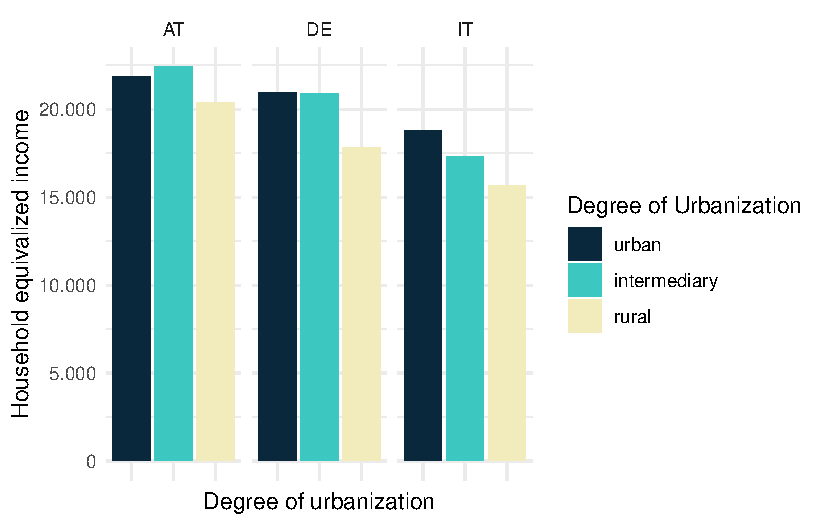
\includegraphics{unit4-draft_files/figure-pdf/fig-degurba-heqinc-1.pdf}

}

\caption{\label{fig-degurba-heqinc}Mean equivalized household income by
country and DEGURBA.}

\end{figure}%

\subsection{Practice time}\label{practice-time}

So now it's time for you to practice. Make a plot, where you have income
on the y axis, and employment hours on the x axis. There should be 3
different lines, one for each country. The year we are doing this for is
2013.

\begin{figure}

\centering{

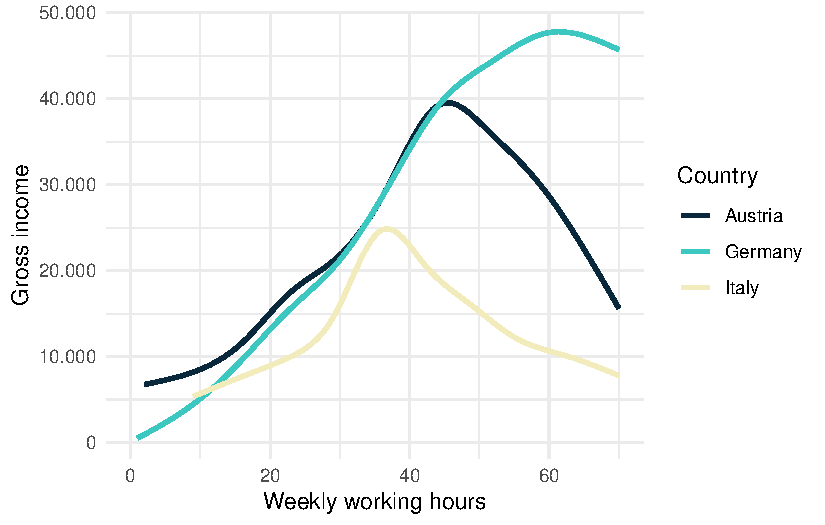
\includegraphics{unit4-draft_files/figure-pdf/fig-employment-income-1.pdf}

}

\caption{\label{fig-employment-income}Income by employment hours, 2013.}

\end{figure}%

\subsection{Export}\label{export}

\subsubsection{Export the data}\label{export-the-data}

For exporting data, we usually use \texttt{write.csv2} or
\texttt{saveRDS}.

\subsubsection{Export the plot}\label{export-the-plot}

You can either manually save a plot or use the \texttt{ggsave} function
of the ggplot package (if your plot is a ggplot).

The \texttt{ggsave} function is a bit complicated, which is because of
the dpi argument. It tells you the resolution of your plot. High
resolutions (dpi = 300 is standard) is good, but make sure to put in
high values for width and hight as well. Also make sure your background
is ``white''.

\begin{Shaded}
\begin{Highlighting}[]
\FunctionTok{ggsave}\NormalTok{(}\FunctionTok{paste0}\NormalTok{(parent\_path, }\StringTok{"/outputs/heqinc{-}degurba.png"}\NormalTok{),}
       \AttributeTok{plot =}\NormalTok{ plot,}
       \AttributeTok{dpi =} \DecValTok{250}\NormalTok{,}
       \AttributeTok{width =} \DecValTok{1440}\NormalTok{,}
       \AttributeTok{height =} \DecValTok{810}\NormalTok{,}
       \AttributeTok{units =} \StringTok{"px"}\NormalTok{,}
       \AttributeTok{bg =} \StringTok{"white"}\NormalTok{)}
\end{Highlighting}
\end{Shaded}

\subsubsection{Export a LaTeX table}\label{export-a-latex-table}

Sometimes, we want our tables to be further used as a LaTeX code. The
typical way to go is by using the \texttt{stargazer} package and
function.

\begin{Shaded}
\begin{Highlighting}[]
\NormalTok{stargazer}\SpecialCharTok{::}\FunctionTok{stargazer}\NormalTok{(df)}
\end{Highlighting}
\end{Shaded}

\begin{verbatim}

% Table created by stargazer v.5.2.3 by Marek Hlavac, Social Policy Institute. E-mail: marek.hlavac at gmail.com
% Date and time: Di, Mai 06, 2025 - 17:32:14
